%!TEX root=thesis.tex

\chapter{Introduction}
\label{cha:intro}

Observations of the sky in different wavelengths have lead to remarkable
discoveries and enhanced our knowledge of the universe, but with the development
of ever more powerful telescopes and data collection methods, we have already
reached a point where there is simply too much astronomical data to process and
analyse by hand. The scale of modern astronomical surveys is enormous. Faint
Images of the Radio Sky at Twenty Centimeters (FIRST) \citep{becker95}, which
began collecting data as early as 1993, detected around 946 000 distant radio
objects; the AllWISE catalogue \citep{cutri13}, released in 2013, contains over
747 million mid-infrared objects.

Despite this, even better telescopes are still being developed. It is a
particularly exciting time in radio astronomy: The Square Kilometre Array (SKA)
is expected to be built by 2024 \citep{ska}, and it will produce over 160
terabytes of data per second. Due to the scale of the SKA, many pathfinder
projects have been launched to provide testbeds for new technologies to be used
in the SKA and for new ways to handle the data that the SKA will produce. One
such project is the Australian SKA Pathfinder (ASKAP), a radio telescope in
Western Australia. ASKAP will soon be used to conduct the Evolutionary Map of
the Universe (EMU).

EMU will be huge and sensitive, imaging 75\% of the sky at sensitivities 40
times higher than the current largest northern sky radio survey. It is expected
to find 30 times more radio galaxies than we have ever known before, bringing
the total to over 70 million. Manual expert analysis of the EMU data will
clearly be intractable.

\begin{figure}
  \centering
  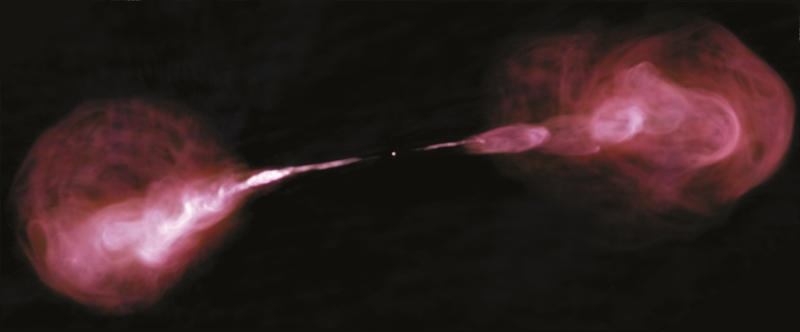
\includegraphics[width=0.8\textwidth]{images/herculesA.jpg}
  \caption{Hercules A, a radio galaxy. We see jets emitted from the supermassive
    black hole near the centre of the image. The galaxy itself is not visible in
    radio wavelengths. \emph{Image: B. Saxton, W. Cotton and R. Perley
    (NRAO/AUI/NSF)}}
  \label{fig:radio-galaxy}
\end{figure}

Objects detected by EMU will need to be cross-identified with their counterparts
in surveys at other wavelengths. Unfortunately, radio objects can be arbitrarily
complex --- many radio objects are jets from supermassive black holes at the
centre of galaxies, and these jets warp as they interact with their environment.
An example of such an object is shown in Figure \ref{fig:radio-galaxy}. An
estimated 10\% of EMU radio objects will be too complicated for current
automated cross-identification algorithms \citep{banfield15, norris11}.

\citet{banfield15} created Radio Galaxy Zoo to attempt to address this
problem. Radio Galaxy Zoo is a citizen science project based on the highly
successful Galaxy Zoo \citep{lintott08, lintott11}. The Zooniverse
platform\footnote{\url{http://zooniverse.org/}} created by Galaxy Zoo provides a
way for non-experts to help researchers label data across a wide range of
scientific fields, and has resulted in well over 110 publications. In the case
of Radio Galaxy Zoo, volunteers are invited to cross-identify radio objects
imaged by the NRAO Very Large Array and the Australia Telescope with their
infrared counterparts imaged by the Wide-area Infrared Survey Explorer (WISE)
and Spitzer telescopes. The cross-identification interface is available online
for anyone to use\footnote{\url{http://radio.galaxyzoo.org/}}. To date, with the
help of thousands of volunteers, Radio Galaxy Zoo has managed to cross-identify
over 100 000 radio galaxies. This still does not compare in scale to EMU, but
the hope is that these cross-identification labels can be used to train
next-generation machine learning algorithms.

This thesis presents a na\"ive, supervised learning approach to the problem of
active galactic nuclei cross-identification, using label data sourced from the
Radio Galaxy Zoo.

\todo{Figure out where to put these acknowledgements. Each of these has an
  acknowledgement requirement, so there's actually a paragraph I have to include
  for each of them.}

This thesis makes use of data products from
\begin{itemize}
    \item ATLAS
    \item WISE
    \item Radio Galaxy Zoo
    \item SWIRE
    \item Breast cancer Wisconsin dataset --- ``The database was obtained from the University of Wisconsin Hospitals, Madison from Dr. William H. Wolberg.''
    \item UCI Machine Learning Repository
\end{itemize}


\section{Contributions of this project}

\begin{itemize}
  \item ML on RGZ
  \item Non-physical model for cross identification
  \item Deep learning features for radio
  \item Effect of features. \url{https://see.stanford.edu/materials/aimlcs229/ml-advice.pdf}
  \item Framing cross identification as object localisation then binary classification
  \item Implementation of Raykar and Yan
  \item Compare Raykar, Yan, MV (wins)
  \item Compare Logistic Regression with Random Forest
  \item Benefit active learning
\end{itemize}
